\section{Brute-Force Attack Modeling} \label{sec:3symbolic-modeling}

% In the previous section, we introduced the verification tool, \Tamarin{}, in detail.
In this section, we will discuss the limitations of existing models and introduce our methodology for capturing brute force behaviors in a general manner.

\subsection{Threat Model and Low-Entropy Adversary} \label{sec:threat-model}

Our adversary extends the classical Dolev-Yao attacker~\cite{dolev1983security}
with a bounded brute-force capability.
As in the Dolev-Yao model, the attacker fully controls the public network: they can intercept, drop, reorder, forge, and replay messages, and they can derive any term that is the result of applying a public function to knowledge already in their possession.
Beyond these capabilities, the attacker may attempt to recover the value of a term $k$ from a function output $f(\ldots, k, \ldots)$ whenever (i)~$k$ has been labeled as low-entropy in the protocol model, and (ii)~every non-$k$ argument of $f$ is either a constant or derivable by the Dolev-Yao attacker.
The recovery is forward: the attacker recomputes $f$ for each candidate value of $k$
and keeps the one whose output matches the observed one exactly.

Such a recovery takes up to $2^{|k|}$ trials, where $|k|$ is the nominal bit-length of $k$,
and is admitted only if $|k|$ lies within a budget fixed in advance by the modeler.
To anchor that budget at a concrete bit level we introduce two graded adversaries used throughout the case studies.
A \emph{semi-attacker} (SA) is budgeted to $\lambda_{\mathrm{SA}} = 64$ bits and can therefore brute-force any key up to 8 bytes in length, matching the computational scale of the documented KNOB attack.
A \emph{quart-attacker} (QA) is budgeted to $\lambda_{\mathrm{QA}} = 32$ bits and can brute-force any key up to 4 bytes, representing a lower-resource adversary.
Both adversaries retain the full Dolev-Yao repertoire in addition to their brute-force oracle; the difference is purely the maximum $|k|$ at which the oracle is allowed to fire.
Sections~\ref{sec:4extension-and-compilation} and~\ref{sec:5case-study} formalize this behavior as multiset-rewriting rules and instantiate SA/QA against concrete BC device configurations.

\subsection{Key-Breaking Oracles}

\emph{Perfect encryption assumption} adopted by current symbolic models prevent adversaries from obtaining any information from the ciphertext.
\cite{cremers2023aead,shi2023blesc,claverie2023tamarin} proposed their methods to loosen this assumption by introducing a set of special rules.
These rules model the behaviors of attackers accessing an oracle, thereby allowing them to obtain certain keys.
% An example of such a rule is as follows:
Such a rule of \cite{claverie2023tamarin} is as follows:
\begin{flalign*}
    \text{\ruleNameText{Rul}} & \text{\ruleNameText{e Oracle}} :                    &\\
    \TFacts{ &\text{\TFact{LowEntropyf4}}(pk1, pk2, n, s), \\
    &\text{\TFact{In}}(pk1), \text{\TFact{In}}(pk2), \text{\TFact{In}}(n), \text{\TFact{In}}(f4(pk1, pk2, n, s))} \TEmpActFact{ } \\
    \TFacts{ &\text{\TFact{Out}}(s)}    
\end{flalign*}
In this rule, the fact \TFact{LowEntropyf4} indicates that the last input $s$ of the function $f4$ possesses a low entropy.
Attackers can recover the value of $s$ by providing all other inputs of $f4$ and its output.
This rule is intuitive and checks the three essential prerequisites for a brute-force attack: knowledge of the function, knowledge of all inputs except the key, and knowledge of the computation result. 
It effectively captures brute-force attacks targeting the $f4$ function.

However, this is not a general modeling method.
The design of this rule implicitly relies on a critical hypothesis: an attacker is capable of, and restricted to, exploiting the function $f4$ to execute a brute force attack on the low-entropy variable $s$.
This hypothesis is confirmed manually, rather than automatically.
This presents a challenge, as the inability to ascertain which function an attacker might utilize to brute force the key renders the application of such a rule infeasible.

To generally capture all brute force attacks, we designed a key-breaking oracle.
This oracle accepts any function and is capable of returning the value of the low-entropy key, provided that the attacker can furnish the function output along with the values of all other relevant variables, as shown below:
\begin{figure}[h]
    \centering
    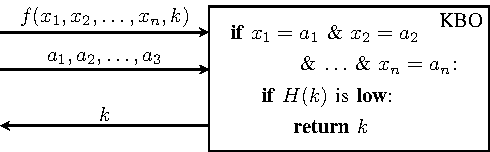
\includegraphics[width=0.7755\columnwidth]{img/general-oracle} 
\end{figure}

% 为了建模这个oracle，我们首先要克服两个困难：
% 函数的不确定性：作为一个通用的oracle，需要能够接收任意的函数输出。在符号模型中，函数符号的匹配都是精确的，不存在模糊匹配的情况。
% 其他参数的不确定性：由于可能收到任意的函数输出，oracle需要根据收到的函数动态地判断还需要哪些其他的输入。
% To model this oracle, two challenges must be overcome:
% \begin{enumerate}
%     \item \textbf{Function Uncertainty:} As a general oracle, it needs to accept the output of any function. In symbolic models, the matching of function symbols is exact, with no fuzzy matching.
%     \item \textbf{Input Uncertainty:} Since any function output may be received, the oracle must dynamically determine which other inputs are required based on the received function.
% \end{enumerate}

\noindent
To model this oracle, there are two challenges.
\begin{enumerate}[leftmargin=*]
    \item \textbf{Uncertainty of Received Functions:} As a general oracle, it should accept any function. 
    But in symbolic models, function symbol matching is precise, prohibiting using a single function symbol to generally match all functions.
    \item \textbf{Uncertainty of Additional Inputs:} Given the uncertainty regarding which function will be received, the oracle must dynamically accommodate additional inputs contingent upon the specific function it encounters.
\end{enumerate}
To address the first challenge, we introduce the concept of message derivation relationships as a substitute for specific function symbols. 
This concept will be explained in detail in \autoref{sec:oracle-modeling}.
To overcome the second, we introduce two more fundamental oracles: the value-breaking oracle and the relationship-breaking oracle. 

% a value-breaking oracle and an algorithm-breaking oracle.
\subsubsection{Value-Breaking Oracle}
% The value-breaking oracle grants attackers the capability to break low-entropy keys, assuming the attacker can identify a computation result of a function in which a low-entropy key is the only input.
The execution process of the value-breaking oracle is delineated as follows:
\begin{figure}[h]
    \centering
    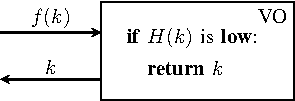
\includegraphics[width=0.4653\columnwidth]{img/oracle1} 
\end{figure}

\noindent The value-breaking oracle grants attackers the capability to break low-entropy keys, assuming the attacker can identify a computation result of a function in which a low-entropy key is the only input. 
An attacker submits to the value-breaking oracle the output of such a function output.
The only thing the value-breaking oracle needs to do is to verify whether the key possesses a low entropy and return the key's value if it does.

\subsubsection{Relationship-Breaking Oracle}
The relationship-breaking oracle is designed to eliminate the attacker's known variables from the key's computation.
The execution process of the relationship-breaking oracle is shown as follows:
\begin{figure}[h]
    \centering
    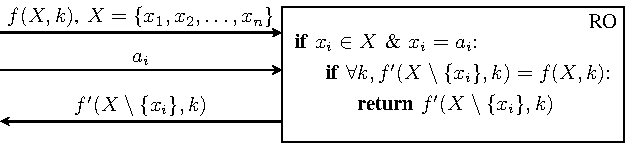
\includegraphics[width=0.99\columnwidth]{img/oracle2} 
\end{figure}

% \noindent Given that an attacker can provide a function $f$ that incorporates a key $k$ and another input variable $x_i$, the oracle can identify another function $f'$ that excludes $x_i$.
% 给定一个函数f，攻击者获得了一个函数输出f(X, k), 其中k是目标密钥，X是除了k之外的所有其他变量的集合。
% 如果攻击者得知X中的某个变量x_i的值，和f(X, k)一起提供给RO，RO会找到一个函数f', 使得f'(k) = f(X, k)，并返回.
\noindent
Given a function $f$ where an attacker acquires the function output $f(X, k)$, in which $k$ represents the target key and $X$ denotes the set of all other input variables excluding $k$. 
If the attacker knows the value of $x_i$, $x_i \in X$ and submits it together with $f(X, k)$ to the relationship-breaking oracle, the oracle will return a new function $f'$ where $f'(X \backslash \{x_i\}, k) = f(X, k)$.
Attackers can access this oracle multiple times until all other input variables are eliminated, except for the target key.
They then utilize the value-breaking oracle to obtain the value of the low-entropy key.


\subsection{Oracle Modeling} \label{sec:oracle-modeling}

We model the previous oracles through a series of rules.
To abstract the process of message derivation within the relationship-breaking oracle, we introduce the concept of message derivation facts, replacing specific function symbols.
Furthermore, to model the relationship-breaking oracle, it is necessary to incorporate message derivation rules that enable the oracle to deduce all message derivation facts visible from the attacker's perspective.
Building on this foundation, we will present our approach to modeling the value-breaking oracle.

\subsubsection{Message Derivation Fact} In the formalization of the relationship-breaking oracle, key computation is abstracted into derivation relationships, represented by message derivation facts.
Each derivation fact maps one message to another.
Specifically, for a one-arity function $f$ and an argument $x$, $f$ can be abstracted as the fact $\text{\TFact{MDerive}}(x, f(x))$.
For the sake of consistency, multi-arity functions are modeled as:
\[
    \text{\TFact{MDerive}}(\langle x_1, x_2, ..., x_n \rangle, f(\langle x_1, x_2, ..., x_n \rangle)),
\]
where $\langle \cdot \rangle$ denotes a function of $n$ arguments, representing the concatenation of $n$ function arguments.
Similarly, a composite function $f \circ g$ can be modeled as the message derivation fact $\text{\TFact{MDerive}}(x, f(g(x)))$.

The relationship-breaking oracle maintains a collection of all functions.
Once a derivation relationship between two messages is identified, the oracle can locate the specific mapping function.
If the oracle needs to identify a function where a certain key $k$ is the sole argument, it suffices to find the fact $\text{\TFact{MDerive}}(k, m)$,
where $m$ is a message derived from $k$.

\subsubsection{Message Derivation Rule}  
Upon the initiation of the attacker's access to the oracle, the oracle acquires all derivation facts present in the current execution process of the protocol.
It then infers all existing derivation facts that are computable from the attacker's perspective.

Formally, given a set $ df_\mathcal{O} $ denotes all message derivation facts known to the oracle, while $ dm_\mathcal{A} $ represents the set of all deducible messages that the adversary can know.
When the adversary $ \mathcal{A} $ initiates interaction with the oracle $ \mathcal{O} $, the oracle gathers all message derivation facts from the current execution of the protocol $\mathcal{P}$, denoted by $df_\mathcal{P}$, and uses these to initialize $ df_\mathcal{O} $.
The set $ df_\mathcal{O} $ is inductively defined by the following rules:
\begin{align*}
    &\infer
        {\text{\TFact{MDer}}(m_1, m_2) \in df_\mathcal{O}}
        {\text{\TFact{MDer}}(m_1, m_2) \in df_\mathcal{P}}
    &&
    \infer
        {\text{\TFact{MDer}}(m_2, m_3) \in df_\mathcal{O}}
        {\begin{array}{c} 
            m_1 \in dm_\mathcal{A} \\ 
            \text{\TFact{MDer}}(\langle m_1, m_2 \rangle, m_3) \in df_\mathcal{O}
        \end{array}}
        % \end{array}} \\[1em]
\end{align*}
\begin{align*}
    &\infer
        {\text{\TFact{MDer}}(m_1, m_3) \in df_\mathcal{O}}
        {\begin{array}{c} 
            \text{\TFact{MDer}}(m_1, m_2) \in df_\mathcal{O} \\ 
            \text{\TFact{MDer}}(m_2, m_3) \in df_\mathcal{O}
        \end{array}} 
    &&
    \infer
        {\text{\TFact{MDer}}(m_1, m_3) \in df_\mathcal{O}}
        {\begin{array}{c} 
            m_2 \in dm_\mathcal{A} \\ 
            \text{\TFact{MDer}}(\langle m_1, m_2 \rangle, m_3) \in df_\mathcal{O}
        \end{array}}
\end{align*}

% These rules, if written in the format of multiset rewriting rules, would look like this:
% \begin{flalign*}
%     \text{\ruleNameText{Rul}} & \text{\ruleNameText{e OracleMsgDerive1}} :                               &\\
%     \TFacts{ &\text{\TFact{MDerive}}(m_1, m_2), \text{\TFact{MDerive}}(m_2, m_3) } \TEmpActFact \\
%     \TFacts{ &\text{\TFact{MDerive}}(m_1, m_3) }        
%     \\
%     \text{\ruleNameText{Rul}} & \text{\ruleNameText{e OracleMsgDerive2}} :                               &\\
%     \TFacts{ &\text{\TFact{MDerive}}(\langle m_1, m_2 \rangle, m_ 3), \text{\TFact{In}}(m_1) } \TEmpActFact \\
%     \TFacts{ &\text{\TFact{MDerive}}(m_2, m_3) }
%     \\
%     \text{\ruleNameText{Rul}} & \text{\ruleNameText{e OracleMsgDerive3}} :                               &\\
%     \TFacts{ &\text{\TFact{MDerive}}(\langle m_1, m_2 \rangle, m_3), \text{\TFact{In}}(m_2) } \TEmpActFact \\
%     \TFacts{ &\text{\TFact{MDerive}}(m_1, m_3) }
% \end{flalign*}
\noindent
In these rules, the attacker is required to continuously supply all known terms to assist the oracle in inferring all visible derivation facts.

\subsubsection{Value-Breaking Oracle} 
% oracle 破解密钥的最后一步，检查目标的key是否是低熵，且攻击者掌握其作为唯一变量的函数输出，如果是，oracle会返回该密钥的数值。这个规则如下：
% 其中，k是攻击者的目标密钥，m是密钥的计算结果，$\text{\TFact{LowEntropy}}(k)$表示k是低熵密钥，在建模具体协议时被手动指定。
In the concluding step of the oracle's key-breaking process, the oracle verifies whether the target key possesses a low entropy and whether the attacker has knowledge of a calculation result where the key is the only variable.
If these prerequisites are satisfied, the oracle will return the value of the key.
This rule can be stated as follows:
\begin{flalign*}
    \text{\ruleNameText{Rul}} & \text{\ruleNameText{e OracleKeyCrack}} :                               &\\
    \TFacts{ &\text{\TFact{MDerive}}(k, m), \text{\TFact{LowEntropy}}(k), \text{\TFact{In}}(m) } \TEmpActFact{ }  \\
    \TFacts{ &\text{\TFact{Out}}(k) }        
\end{flalign*}
where $k$ denotes the attacker's target key, $m$ represents the computation result from the key, and $\text{\TFact{LowEntropy}}(k)$ labels that $k$ is a low-entropy key, which is specified during modeling a certain protocol.
% Such a fact is essential for the oracle to determine whether the key's entropy is low.
